\paragraph{Blogger}\mbox{}\\
\begin{wrapfigure}{l}{7cm}
    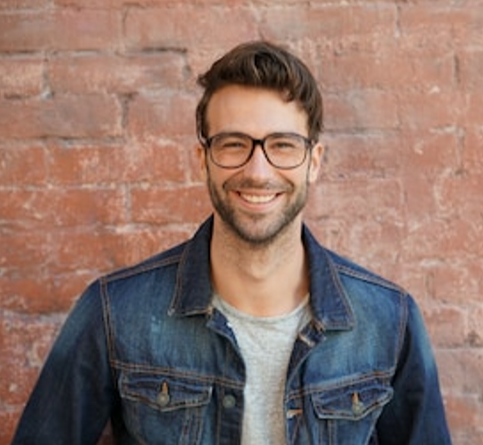
\includegraphics[scale=0.68]{studio-fattibilità/francesco}
    \caption{Foto fantasiosa della persona Roberto}
\end{wrapfigure}
Roberto è un uomo di 30 anni, che dopo aver terminato gli studi presso il liceo scientifico ha deciso di viaggiare in giro per l'Europa per un anno. Roberto soffre di deuteranopia (tipologia di daltonismo). Durante quest'anno ha conosciuto la sua attuale ragazza ed ora vivono assieme in un paesino vicino a Bellinzona. Roberto, grazie alle sue conoscenze informatiche ha creato un blog e ha aperto un canale \textit{YouTube}. I contenuti che produce trattano di attualità ed è seguito da un vasto pubblico di ragazzi tra i 16 e i 25 anni. Nel suo appartamento ha una stanza interamente dedicata alla realizzazione dei video che poi pubblica sul suo canale \textit{YouTube}, in questa stanza trova anche spazio una scrivania con 2 monitor da 27'' e un computer fisso di ultima generazione. Per aggiornare il suo blog utilizza \textit{WordPress} che ormai non ha più segreti per lui.\\ 
Da Marzo 2019 ha iniziato una rubrica settimanale nella quale racconta l'evoluzione della situazione epidemiologica in Italia e nel mondo, che segue con rigore scientifico, al fine di riuscire a spiegare in maniera semplice e accurata i difficili dati che i giornali divulgano. Utilizza diverse fonti per raccogliere i dati e svariati strumenti per analizzarli. 
\begin{itemize}
    \item Attitudine:
    \begin{itemize}
        \item mentalità aperta;
        \item volontà di andare a fondo nelle notizie, raccogliendo pareri disparati;
    \end{itemize}
    \item Comportamento: 
    \begin{itemize}
        \item lettura mattutina delle informazioni che monitora nel resto della giornata mediante RSS;
        \item interazione con i suoi follower, ascolto delle loro opinioni e raccolta dei loro interessi, per crearvi nuovi contenuti più attraenti per la sua \textit{community};
    \end{itemize}
    \item Obiettivi (\textit{end goals}): creare contenuti relativi all'epidemia, basando le sue argomentazioni sui dati della dashboard del DPC;
    \item Motivazione (\textit{life goals}): stimolare una libera discussione tra i suoi follower (lettori, ascoltatori, ecc.) sui temi caldi del momento;
    \item Obiettivi del sistema:
    \begin{itemize}
        \item possibilità di esportare elementi grafici in formato immagine o widget HTML da incorporare;
        \item possibilità di selezionare solo alcuni elementi grafici per comporli in una mini dashboard da incorporare; 
        \item ogni grafico deve utilizzare modalità multiple per veicolare informazioni (mouse over per esplicitare contenuto informativo di componenti grafiche, icone, ecc.). 
    \end{itemize}
\end{itemize}